\documentclass[aspectratio=169,10pt]{beamer}
\usetheme{Madrid}
\usecolortheme{seahorse}

\usepackage[utf8]{inputenc}
\usepackage{amsmath, amssymb, amsfonts, mathtools}
\usepackage{listings}
\usepackage{xcolor}
\usepackage{graphicx}
\usepackage{hyperref}

\graphicspath{{figures/}}

% ============================================================================
% Code Listing Setup
% ============================================================================
\lstset{
    basicstyle=\ttfamily\scriptsize,
    keywordstyle=\color{blue}\bfseries,
    commentstyle=\color{green!50!black}\itshape,
    stringstyle=\color{red},
    showstringspaces=false,
    breaklines=true,
    frame=single,
    numbers=left,
    numberstyle=\tiny,
    numbersep=5pt,
    xleftmargin=20pt,
    framexleftmargin=15pt,
}

% ============================================================================
% Theme Customization
% ============================================================================
\setbeamertemplate{footline}[frame number]
\setbeamertemplate{navigation symbols}{}

% ============================================================================
% Title Information
% ============================================================================
\title[Continuous Functions]{Pathak Chapter 1d: Continuous Functions}
\subtitle{Spaces of Continuous Functions, Carathéodory Functions, \\ and Superposition Operators}
\author{Based on: An Introduction to Nonlinear Analysis and Fixed Point Theory (2018)}
\date{\today}

% ============================================================================
% Document
% ============================================================================
\begin{document}

% ============================================================================
% Title Slide
% ============================================================================
\begin{frame}
    \titlepage
\end{frame}

% ============================================================================
% Table of Contents
% ============================================================================
\begin{frame}{Table of Contents}
    \tableofcontents
\end{frame}

% ============================================================================
% Section 1: Introduction to Continuous Functions
% ============================================================================
\section{Introduction to Continuous Functions}

\begin{frame}{What Are Continuous Functions?}
    \begin{definition}[Continuous Function]
        Let $(X, d_X)$ and $(Y, d_Y)$ be metric spaces. A function $f: X \to Y$ is \textbf{continuous} at $x_0 \in X$ if:
        \[
            \forall \epsilon > 0, \exists \delta > 0: d_X(x, x_0) < \delta \implies d_Y(f(x), f(x_0)) < \epsilon
        \]

        $f$ is continuous on $X$ if it is continuous at every point of $X$.
    \end{definition}

    \vspace{0.3cm}
    \textbf{Key Properties:}
    \begin{itemize}
        \item Captures the intuitive notion of ``no jumps''
        \item Preserves limits: $\lim_{n \to \infty} x_n = x \implies \lim_{n \to \infty} f(x_n) = f(x)$
        \item Generalizes from $\mathbb{R}$ to abstract metric and topological spaces
    \end{itemize}
\end{frame}

\begin{frame}{Continuous Functions in Different Spaces}
    \begin{columns}
        \column{0.5\textwidth}
        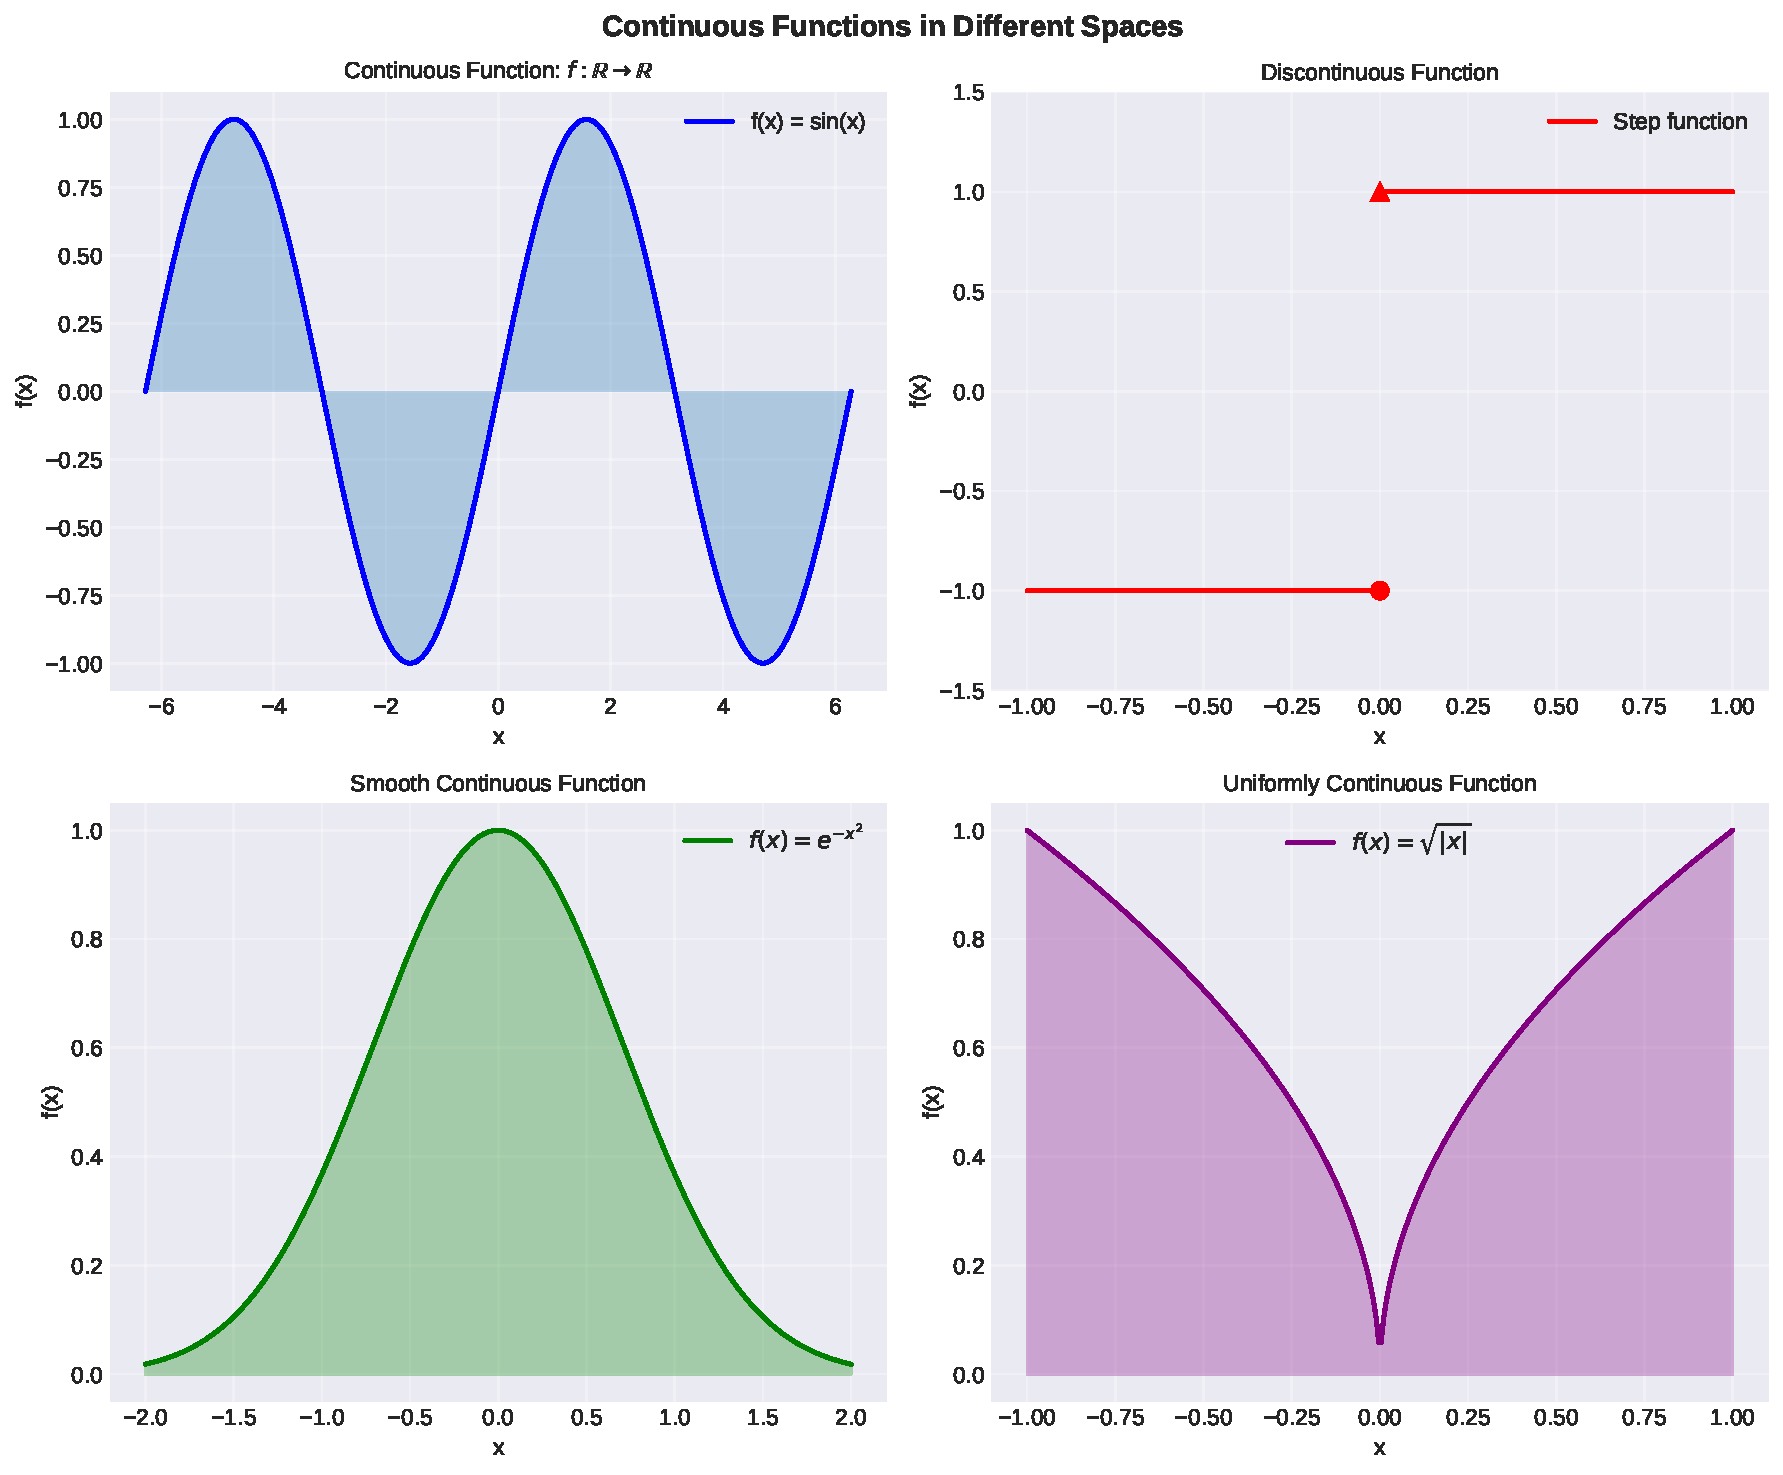
\includegraphics[width=\textwidth]{fig_continuous_functions.pdf}

        \column{0.5\textwidth}
        \textbf{Examples:}
        \begin{itemize}
            \item Polynomial functions: $f(x) = x^2 + 1$
            \item Trigonometric: $f(x) = \sin(x)$
            \item Exponential: $f(x) = e^{-x^2}$
            \item Absolute value: $f(x) = |x|$ (continuous but not smooth)
        \end{itemize}

        \vspace{0.3cm}
        \textbf{Non-examples:}
        \begin{itemize}
            \item Step functions (discontinuous at jumps)
            \item Floor function: $\lfloor x \rfloor$
        \end{itemize}
    \end{columns}
\end{frame}

% ============================================================================
% Section 2: Spaces of Continuous Functions
% ============================================================================
\section{Spaces of Continuous Functions}

\begin{frame}{The Space $C(\Omega)$}
    \begin{definition}[Space of Continuous Functions]
        Let $\Omega$ be a metric space. The space $C(\Omega)$ consists of all continuous, real-valued functions on $\Omega$:
        \[
            C(\Omega) = \{f: \Omega \to \mathbb{R} \mid f \text{ is continuous}\}
        \]
    \end{definition}

    \vspace{0.3cm}
    \textbf{Natural Norm (for bounded $\Omega$):}
    \[
        \|f\|_\infty = \max_{x \in \Omega} |f(x)|
    \]

    \vspace{0.3cm}
    \textbf{Properties of $(C(\Omega), \|\cdot\|_\infty)$:}
    \begin{itemize}
        \item Complete normed space (Banach space)
        \item Separable if $\Omega$ is compact and separable
        \item Reflexive if and only if $\Omega$ is finite
    \end{itemize}
\end{frame}

\begin{frame}[fragile]{Code Example: Checking Continuity in $\mathbb{R}$}
    \begin{lstlisting}[language=Python]
import numpy as np
from scipy.optimize import fminbound

def is_continuous_approx(f, a, b, x0, eps=1e-6, delta_tol=1e-4):
    """
    Approximately check continuity of f at x0 using epsilon-delta definition.
    Returns True if for given epsilon, delta exists.
    """
    # Check if |f(x) - f(x0)| < eps for all x with |x - x0| < delta
    delta = delta_tol
    x_test = np.linspace(x0 - delta, x0 + delta, 100)
    x_test = x_test[(x_test >= a) & (x_test <= b)]

    f_x0 = f(x0)
    f_x = f(x_test)
    max_diff = np.max(np.abs(f_x - f_x0))

    return max_diff < eps

# Test with f(x) = x^2 (continuous)
f = lambda x: x**2
print(is_continuous_approx(f, -1, 1, 0.5))  # True
    \end{lstlisting}
\end{frame}

\begin{frame}{Hierarchy of Function Spaces}
    \begin{columns}
        \column{0.6\textwidth}
        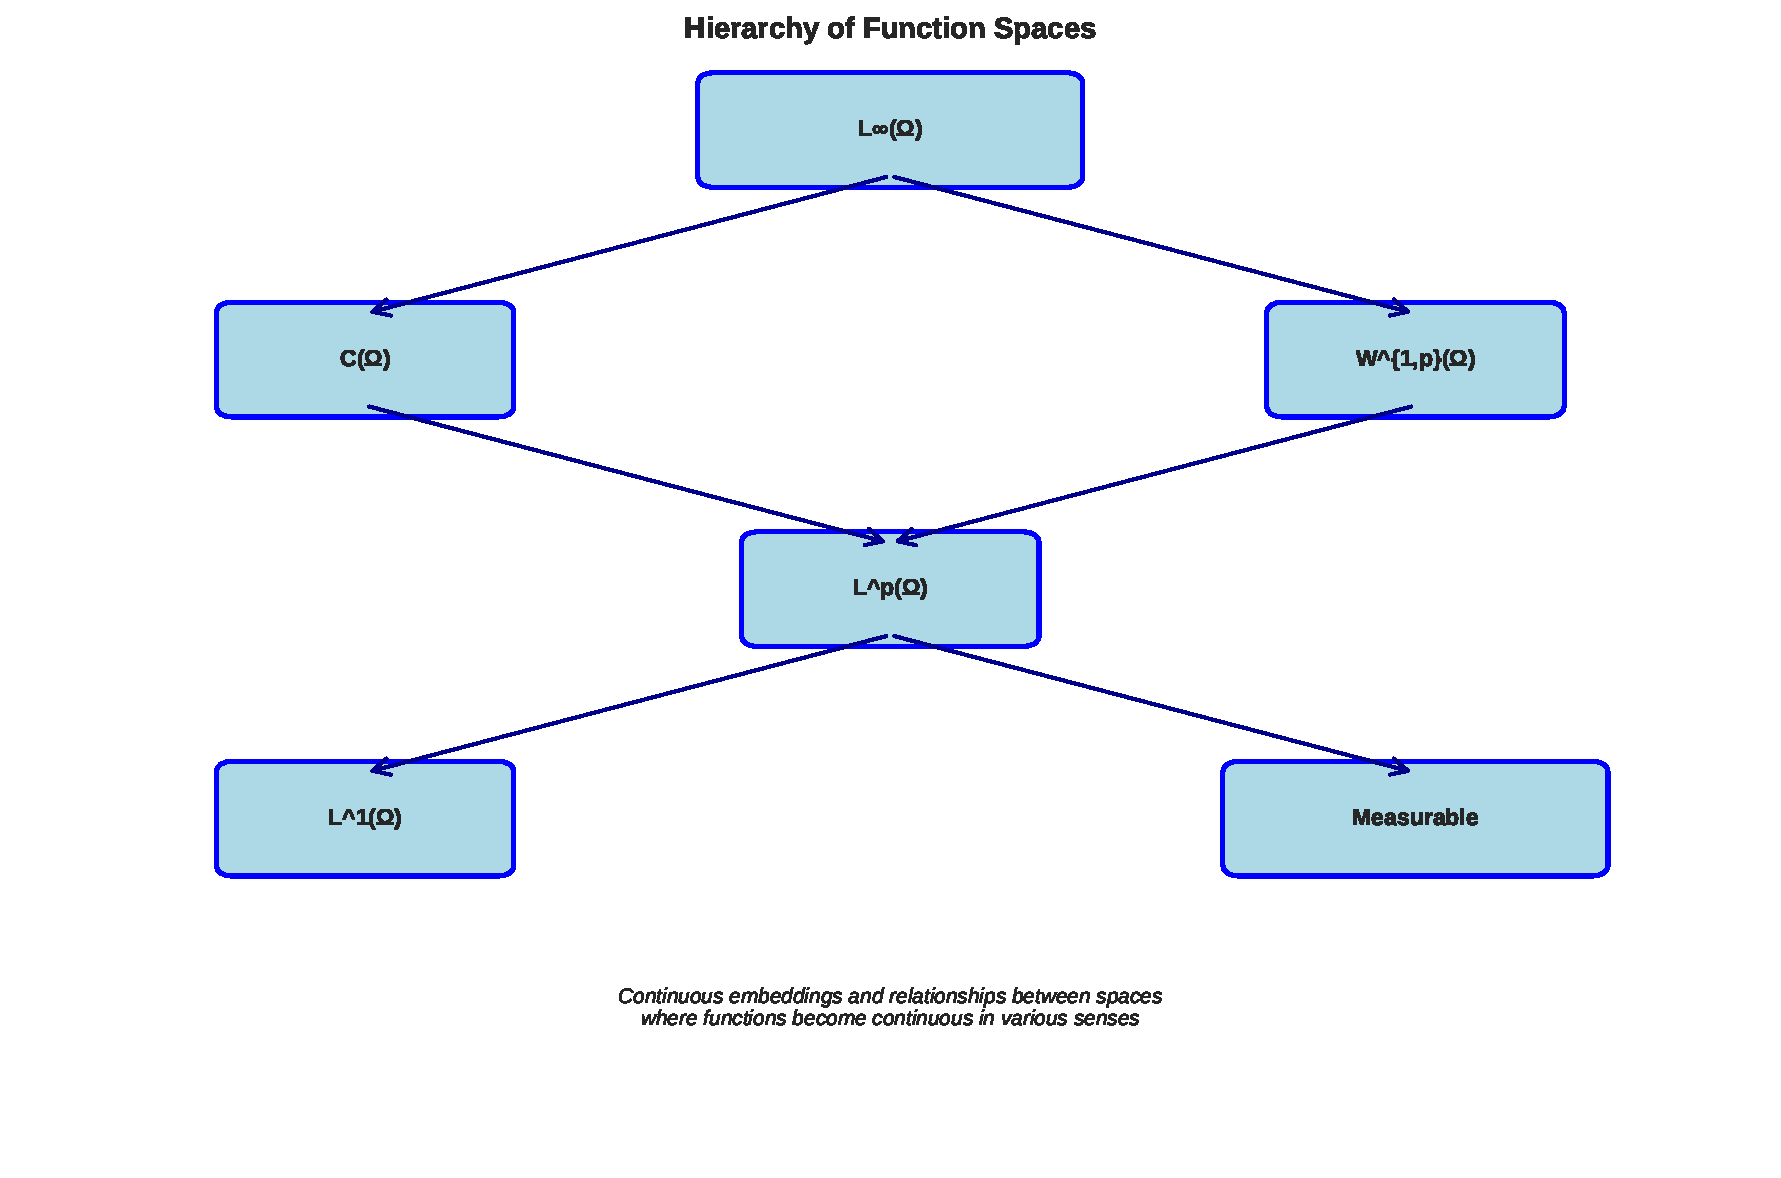
\includegraphics[width=\textwidth]{fig_function_spaces.pdf}

        \column{0.4\textwidth}
        \textbf{Space Relationships:}
        \begin{itemize}
            \item $C(\Omega) \subset L^\infty(\Omega)$
            \item $L^\infty(\Omega) \subset L^p(\Omega)$
            \item $W^{1,p}(\Omega)$ contains functions with weak derivatives
            \item All embed into spaces of measurable functions
        \end{itemize}

        \vspace{0.2cm}
        \small
        (For bounded $\Omega$ with Lebesgue measure)
    \end{columns}
\end{frame}

% ============================================================================
% Section 3: Carathéodory Functions
% ============================================================================
\section{Carathéodory Functions}

\begin{frame}{Carathéodory Functions: Definition}
    \begin{definition}[Carathéodory Function]
        Let $\Omega$ be a measure space and $U$ a metric space. A function $f: \Omega \times U \to \mathbb{R}$ is called a \textbf{Carathéodory function} if:

        \begin{enumerate}
            \item $f(s, \cdot)$ is \textbf{continuous} for almost all $s \in \Omega$
            \item $f(\cdot, u)$ is \textbf{measurable} for all $u \in U$
        \end{enumerate}
    \end{definition}

    \vspace{0.3cm}
    \textbf{Intuition:}
    \begin{itemize}
        \item ``Almost continuous in the second variable''
        \item ``Measurable in the first variable''
        \item Natural condition for existence of solutions to differential equations
    \end{itemize}

    \vspace{0.3cm}
    \textbf{Named after:} Constantin Carathéodory (1873--1950), Greek mathematician
\end{frame}

\begin{frame}{Carathéodory Conditions in Detail}
    \begin{columns}
        \column{0.5\textwidth}
        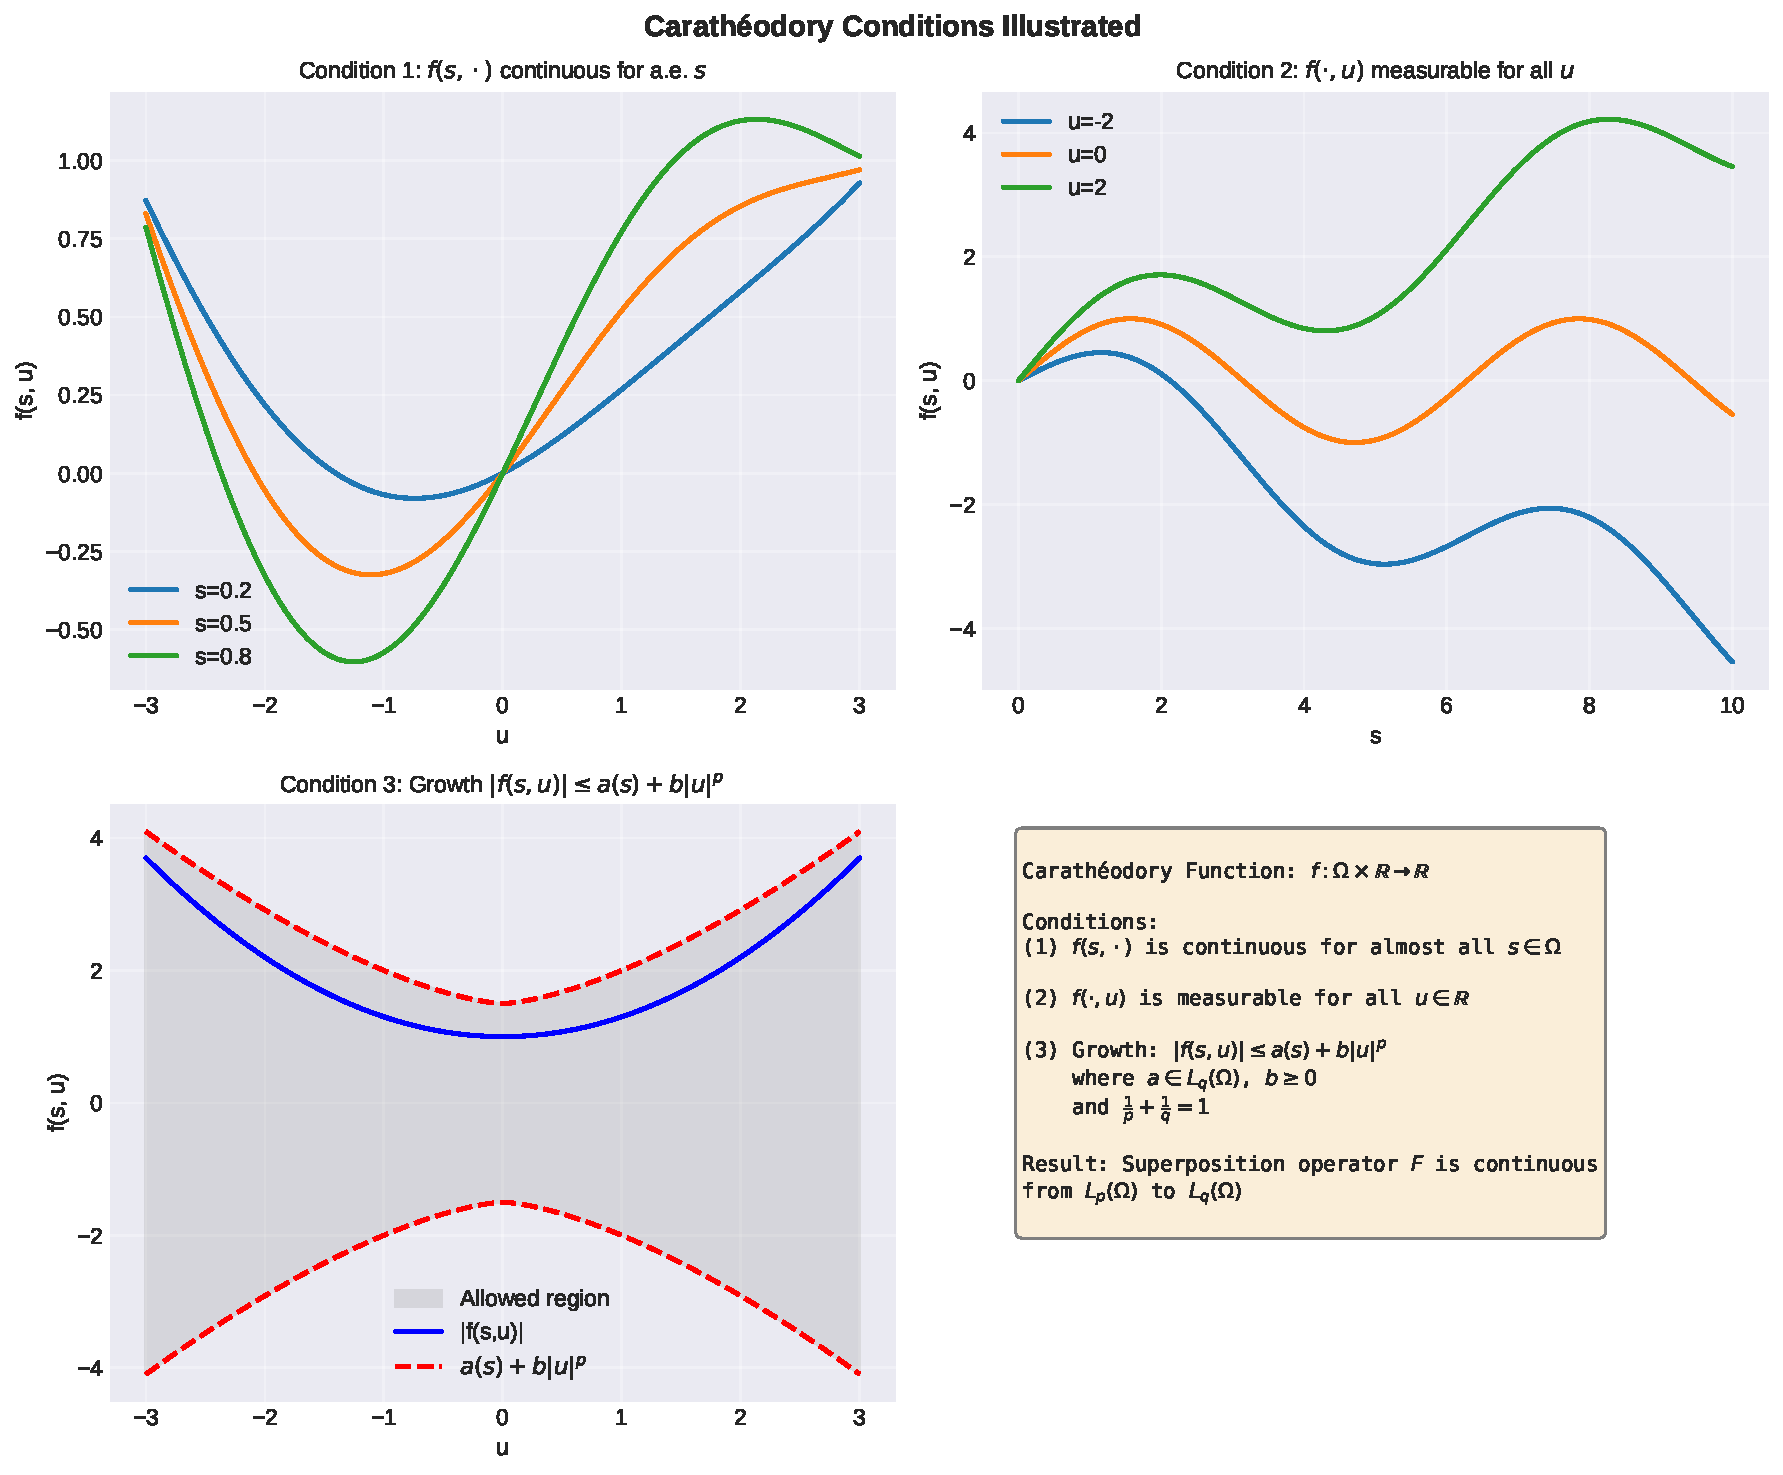
\includegraphics[width=\textwidth]{fig_caratheodory_conditions.pdf}

        \column{0.5\textwidth}
        \textbf{Condition 1:} Continuity in $u$
        \begin{itemize}
            \item For each fixed $s$, the map $u \mapsto f(s,u)$ is continuous
            \item Only needs to hold for almost all $s$
            \item Allows ``bad'' behavior on measure-zero sets
        \end{itemize}

        \vspace{0.3cm}
        \textbf{Condition 2:} Measurability in $s$
        \begin{itemize}
            \item For each fixed $u$, the map $s \mapsto f(s,u)$ is measurable
            \item Essential for integration theory
        \end{itemize}
    \end{columns}
\end{frame}

\begin{frame}{Growth Condition for Carathéodory Functions}
    \textbf{Growth Condition:}
    \[
        |f(s, u)| \leq a(s) + b|u|^p
    \]
    where:
    \begin{itemize}
        \item $a \in L_q(\Omega)$ with $q \geq 1$
        \item $b \geq 0$ is a constant
        \item $p > 0$ controls growth in $u$
        \item $\frac{1}{p} + \frac{1}{q} = 1$ (Hölder conjugates)
    \end{itemize}

    \vspace{0.3cm}
    \textbf{Significance:}
    \begin{itemize}
        \item Ensures the superposition operator $F$ maps $L_p(\Omega)$ into $L_q(\Omega)$
        \item Prevents too-rapid growth in the variable $u$
        \item Necessary for many existence theorems in PDE theory
    \end{itemize}

    \vspace{0.3cm}
    \textbf{Example:} $f(s, u) = a(s) + b|u|$ with $a \in L_q(\Omega)$ satisfies growth with $p=1$
\end{frame}

% ============================================================================
% Section 4: Superposition and Nemytski Operators
% ============================================================================
\section{Superposition and Nemytski Operators}

\begin{frame}{Superposition Operator (Nemytski Operator)}
    \begin{definition}[Superposition Operator]
        Let $f: \Omega \times \mathbb{R} \to \mathbb{R}$ be a function. The \textbf{superposition operator} (or \textbf{Nemytski operator}) generated by $f$ is:
        \[
            F(x)(s) = f(s, x(s)) \quad \text{for } s \in \Omega
        \]
    \end{definition}

    \vspace{0.3cm}
    \textbf{Alternative names:}
    \begin{itemize}
        \item Composition operator
        \item Substitution operator
        \item Outer superposition operator
    \end{itemize}

    \vspace{0.3cm}
    \textbf{Named after:} Vladimir Nemytskii (1900--1967), Soviet mathematician
\end{frame}

\begin{frame}{Nemytski Operator Illustrated}
    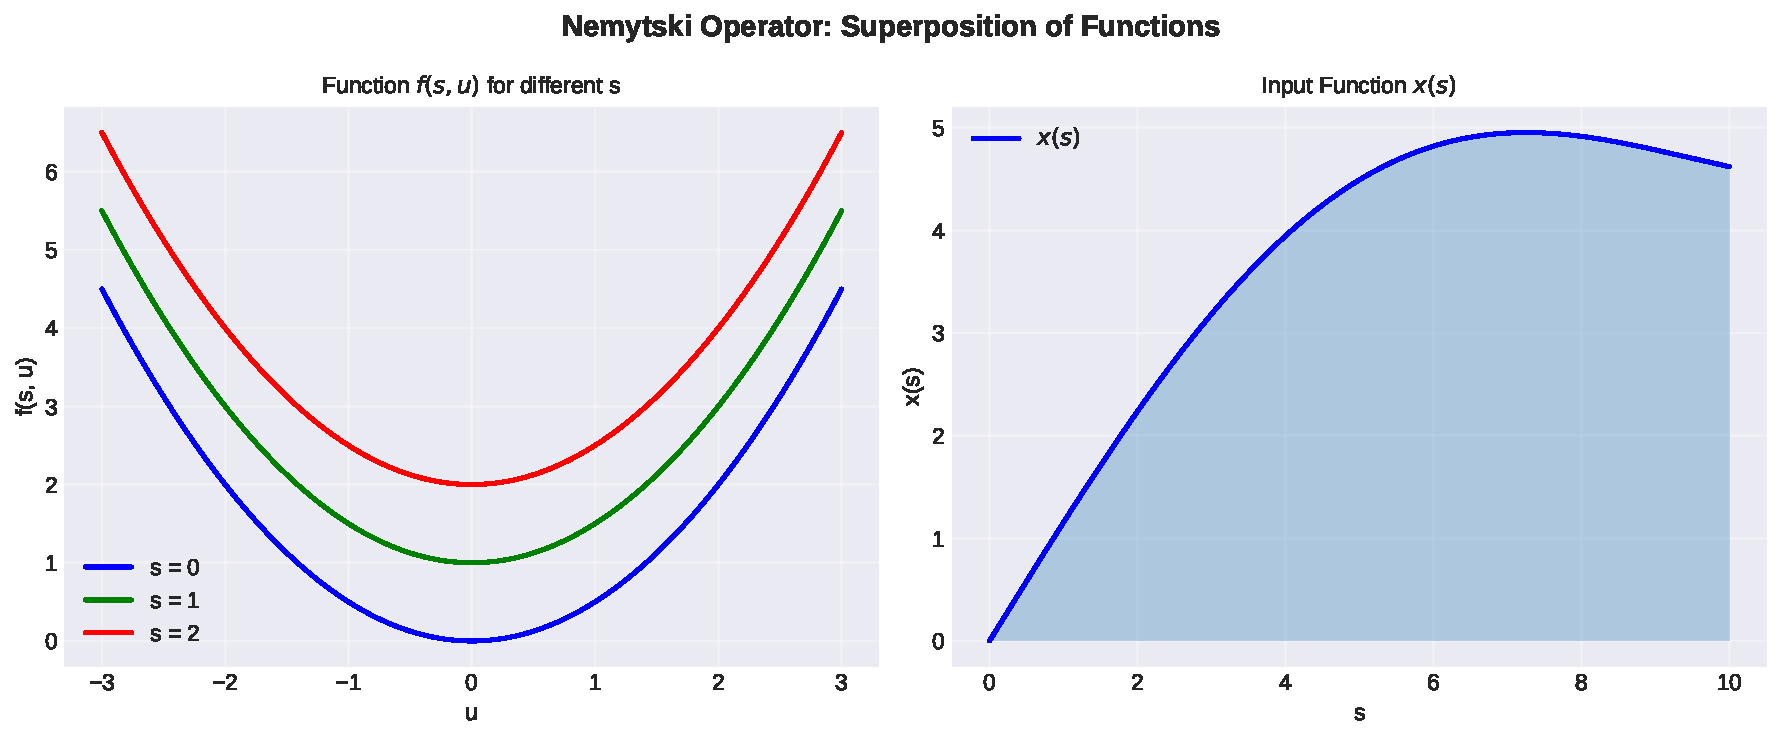
\includegraphics[width=\textwidth]{fig_nemytski_operator.pdf}

    \vspace{0.3cm}
    \small
    \textbf{How it works:}
    \begin{enumerate}
        \item Start with an input function $x: \Omega \to \mathbb{R}$
        \item For each $s \in \Omega$, evaluate $f(s, x(s))$
        \item Result is output function $F(x): \Omega \to \mathbb{R}$
    \end{enumerate}
\end{frame}

\begin{frame}{Continuity of Superposition Operators}
    \begin{theorem}[Continuity of Nemytski Operator]
        Let $f: \Omega \times \mathbb{R} \to \mathbb{R}$ satisfy the Carathéodory conditions. Then the corresponding superposition operator $F$ is continuous and bounded from $L_p(\Omega)$ to $L_q(\Omega)$.
    \end{theorem}

    \vspace{0.3cm}
    \textbf{Key Assumption:} The growth condition
    \[
        |f(s, x)| \leq a(s) + b|x|^{p/q}
    \]
    where $a \in L_q(\Omega)$, $b \geq 0$.

    \vspace{0.3cm}
    \textbf{Consequence:} If $\|x\|_p \to 0$, then $\|F(x)\|_q \to 0$
\end{frame}

\begin{frame}[fragile]{Code Example: Nemytski Operator}
    \begin{lstlisting}[language=Python]
import numpy as np
from scipy.integrate import quad

def nemytski_operator(f, x_func, s_vals, norm='inf'):
    """
    Compute the Nemytski operator F(x)(s) = f(s, x(s))

    Args:
        f: function f(s, u)
        x_func: input function x(s)
        s_vals: evaluation points
        norm: 'inf' for L-infinity or 'p' for L^p norm

    Returns:
        Array of F(x)(s) values
    """
    # Compute F(x)(s) = f(s, x(s)) for each s
    fx = np.array([f(s, x_func(s)) for s in s_vals])
    return fx

# Example: f(s,u) = s + u^2
f = lambda s, u: s + 0.1*u**2
x = lambda s: np.sin(s)

s = np.linspace(0, 2*np.pi, 100)
Fx = nemytski_operator(f, x, s)

# Norm computation
L_inf_norm = np.max(np.abs(Fx))
L_2_norm = np.sqrt(np.mean(Fx**2))

print(f"L-infinity norm: {L_inf_norm:.4f}")
print(f"L^2 norm: {L_2_norm:.4f}")
    \end{lstlisting}
\end{frame}

% ============================================================================
% Section 5: Uniform Continuity
% ============================================================================
\section{Uniform Continuity and Compactness}

\begin{frame}{Uniform Continuity}
    \begin{definition}[Uniform Continuity]
        A function $f: X \to Y$ between metric spaces is \textbf{uniformly continuous} if:
        \[
            \forall \epsilon > 0, \exists \delta > 0: \forall x, y \in X, \quad d_X(x, y) < \delta \implies d_Y(f(x), f(y)) < \epsilon
        \]
    \end{definition}

    \vspace{0.3cm}
    \textbf{Key Difference from Continuity:}
    \begin{itemize}
        \item In continuity: $\delta$ may depend on the point $x_0$
        \item In uniform continuity: $\delta$ works for \textit{all} points simultaneously
        \item Much stronger condition!
    \end{itemize}

    \vspace{0.3cm}
    \textbf{Example:}
    \begin{itemize}
        \item $f(x) = \sin(x)$ on $\mathbb{R}$ is uniformly continuous
        \item $f(x) = \frac{1}{x}$ on $(0,1)$ is continuous but NOT uniformly continuous
    \end{itemize}
\end{frame}

\begin{frame}{Uniform Continuity Visualized}
    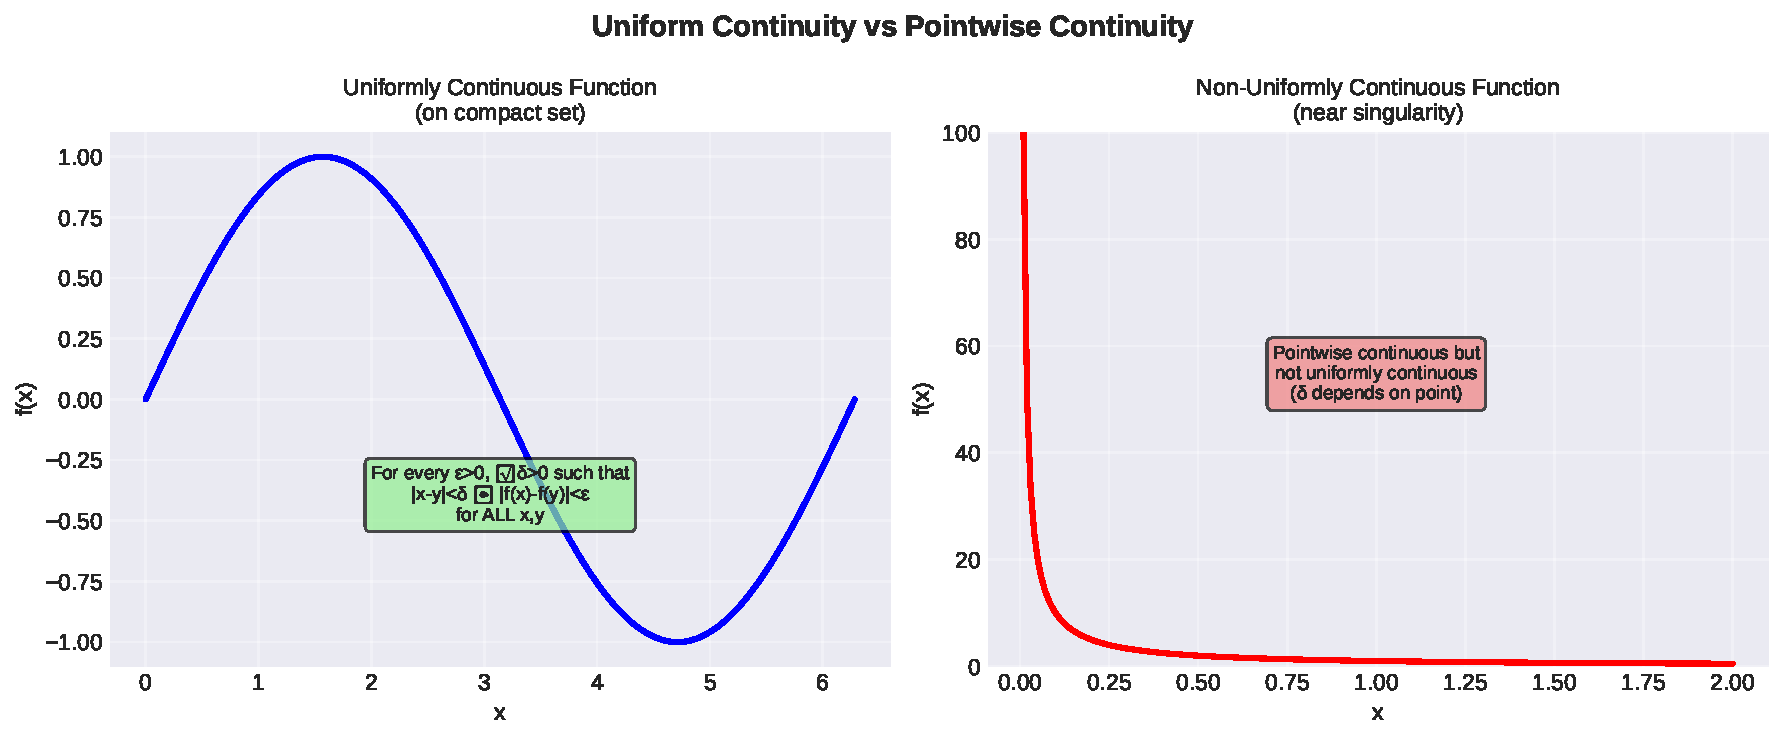
\includegraphics[width=\textwidth]{fig_uniform_continuity.pdf}
\end{frame}

\begin{frame}{Continuous Functions on Compact Sets}
    \begin{theorem}[Continuous Functions on Compact Sets]
        If $K$ is a compact metric space and $f: K \to \mathbb{R}$ is continuous, then:

        \begin{enumerate}
            \item $f(K)$ is compact
            \item $f$ is \textbf{bounded}: $\exists M > 0$ such that $|f(x)| \leq M$ for all $x \in K$
            \item $f$ \textbf{attains its extrema}: $\exists x_{\min}, x_{\max} \in K$ such that
            \[
                f(x_{\min}) = \min_{x \in K} f(x), \quad f(x_{\max}) = \max_{x \in K} f(x)
            \]
            \item $f$ is \textbf{uniformly continuous} on $K$
        \end{enumerate}
    \end{theorem}

    \vspace{0.3cm}
    \textbf{Practical Significance:}
    \begin{itemize}
        \item Ensures optimization problems have solutions
        \item Justifies using numerical methods on compact domains
    \end{itemize}
\end{frame}

\begin{frame}{Continuous Functions on Compact Sets (Illustrated)}
    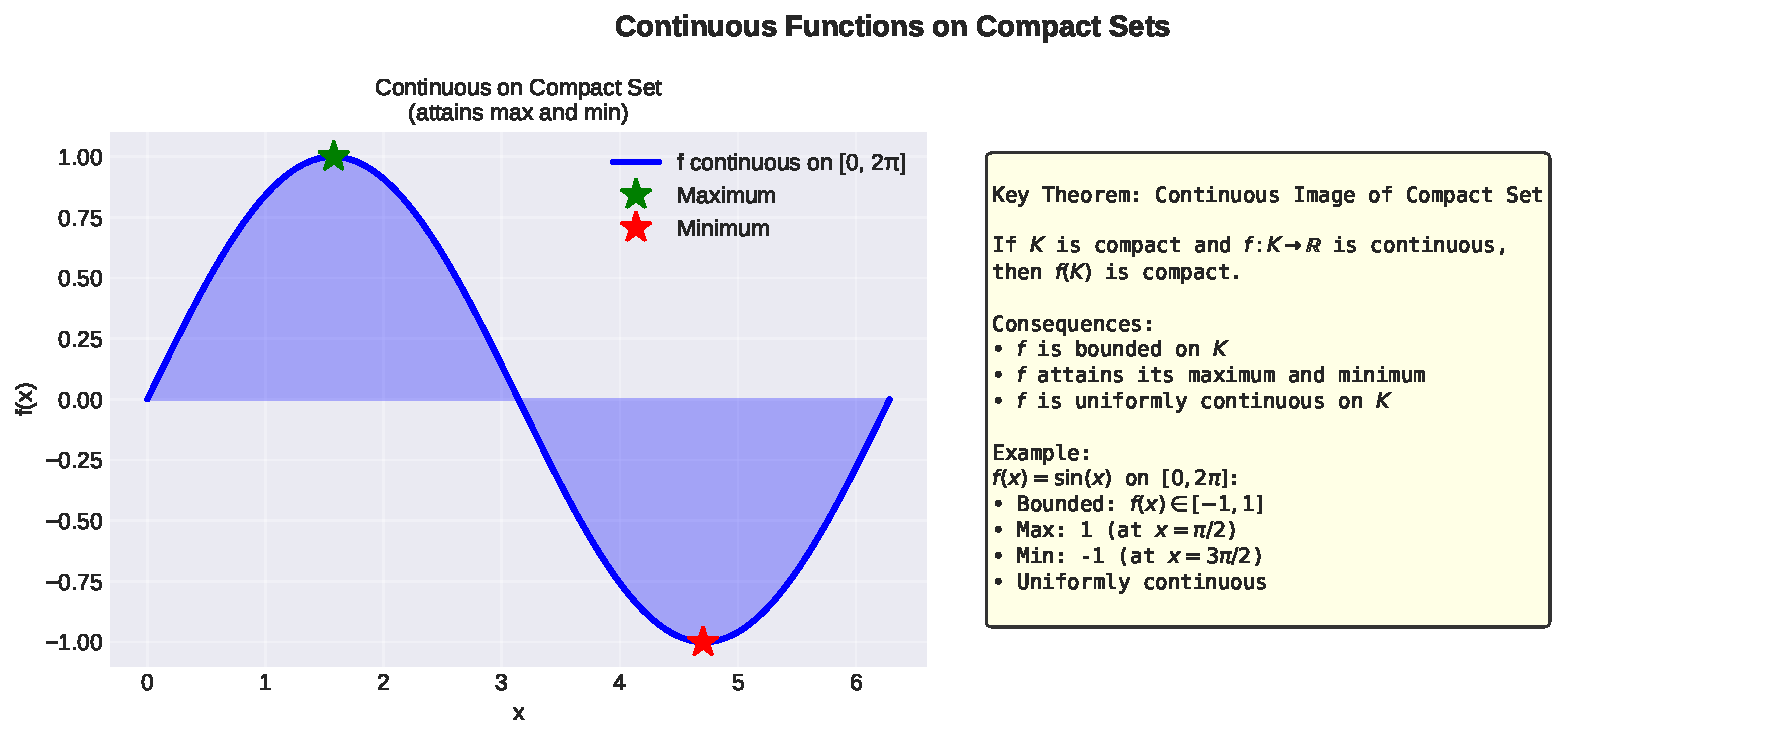
\includegraphics[width=\textwidth]{fig_compactness_continuity.pdf}
\end{frame}

% ============================================================================
% Section 6: Sobolev Spaces
% ============================================================================
\section{Sobolev Spaces and Weak Derivatives}

\begin{frame}{Weak Derivatives}
    \begin{definition}[Weak Derivative]
        Let $u, v \in L^p(\Omega)$ and $\alpha$ a multi-index. We say $v$ is the \textbf{weak partial derivative} $D^\alpha u$ if:
        \[
            \int_\Omega u(x) D^\alpha \varphi(x) \, dx = (-1)^{|\alpha|} \int_\Omega v(x) \varphi(x) \, dx
        \]
        for all test functions $\varphi \in C_0^\infty(\Omega)$ (smooth with compact support).
    \end{definition}

    \vspace{0.3cm}
    \textbf{Advantages:}
    \begin{itemize}
        \item Extends differentiation beyond classical sense
        \item Allows handling of non-smooth functions
        \item Essential for modern PDE theory
        \item Makes spaces complete (Banach spaces)
    \end{itemize}
\end{frame}

\begin{frame}{Sobolev Spaces: Definition and Properties}
    \begin{definition}[Sobolev Space]
        The \textbf{Sobolev space} $W^{k,p}(\Omega)$ is:
        \[
            W^{k,p}(\Omega) = \left\{u \in L^p(\Omega) : D^\alpha u \in L^p(\Omega) \text{ for all } |\alpha| \leq k\right\}
        \]

        Equipped with norm:
        \[
            \|u\|_{k,p} = \left(\sum_{|\alpha| \leq k} \int_\Omega |D^\alpha u|^p \, dx\right)^{1/p}
        \]
    \end{definition}

    \vspace{0.3cm}
    \textbf{Special case $p = 2$:} $H^k(\Omega) = W^{k,2}(\Omega)$ is a Hilbert space
\end{frame}

\begin{frame}{Sobolev Spaces (Illustrated)}
    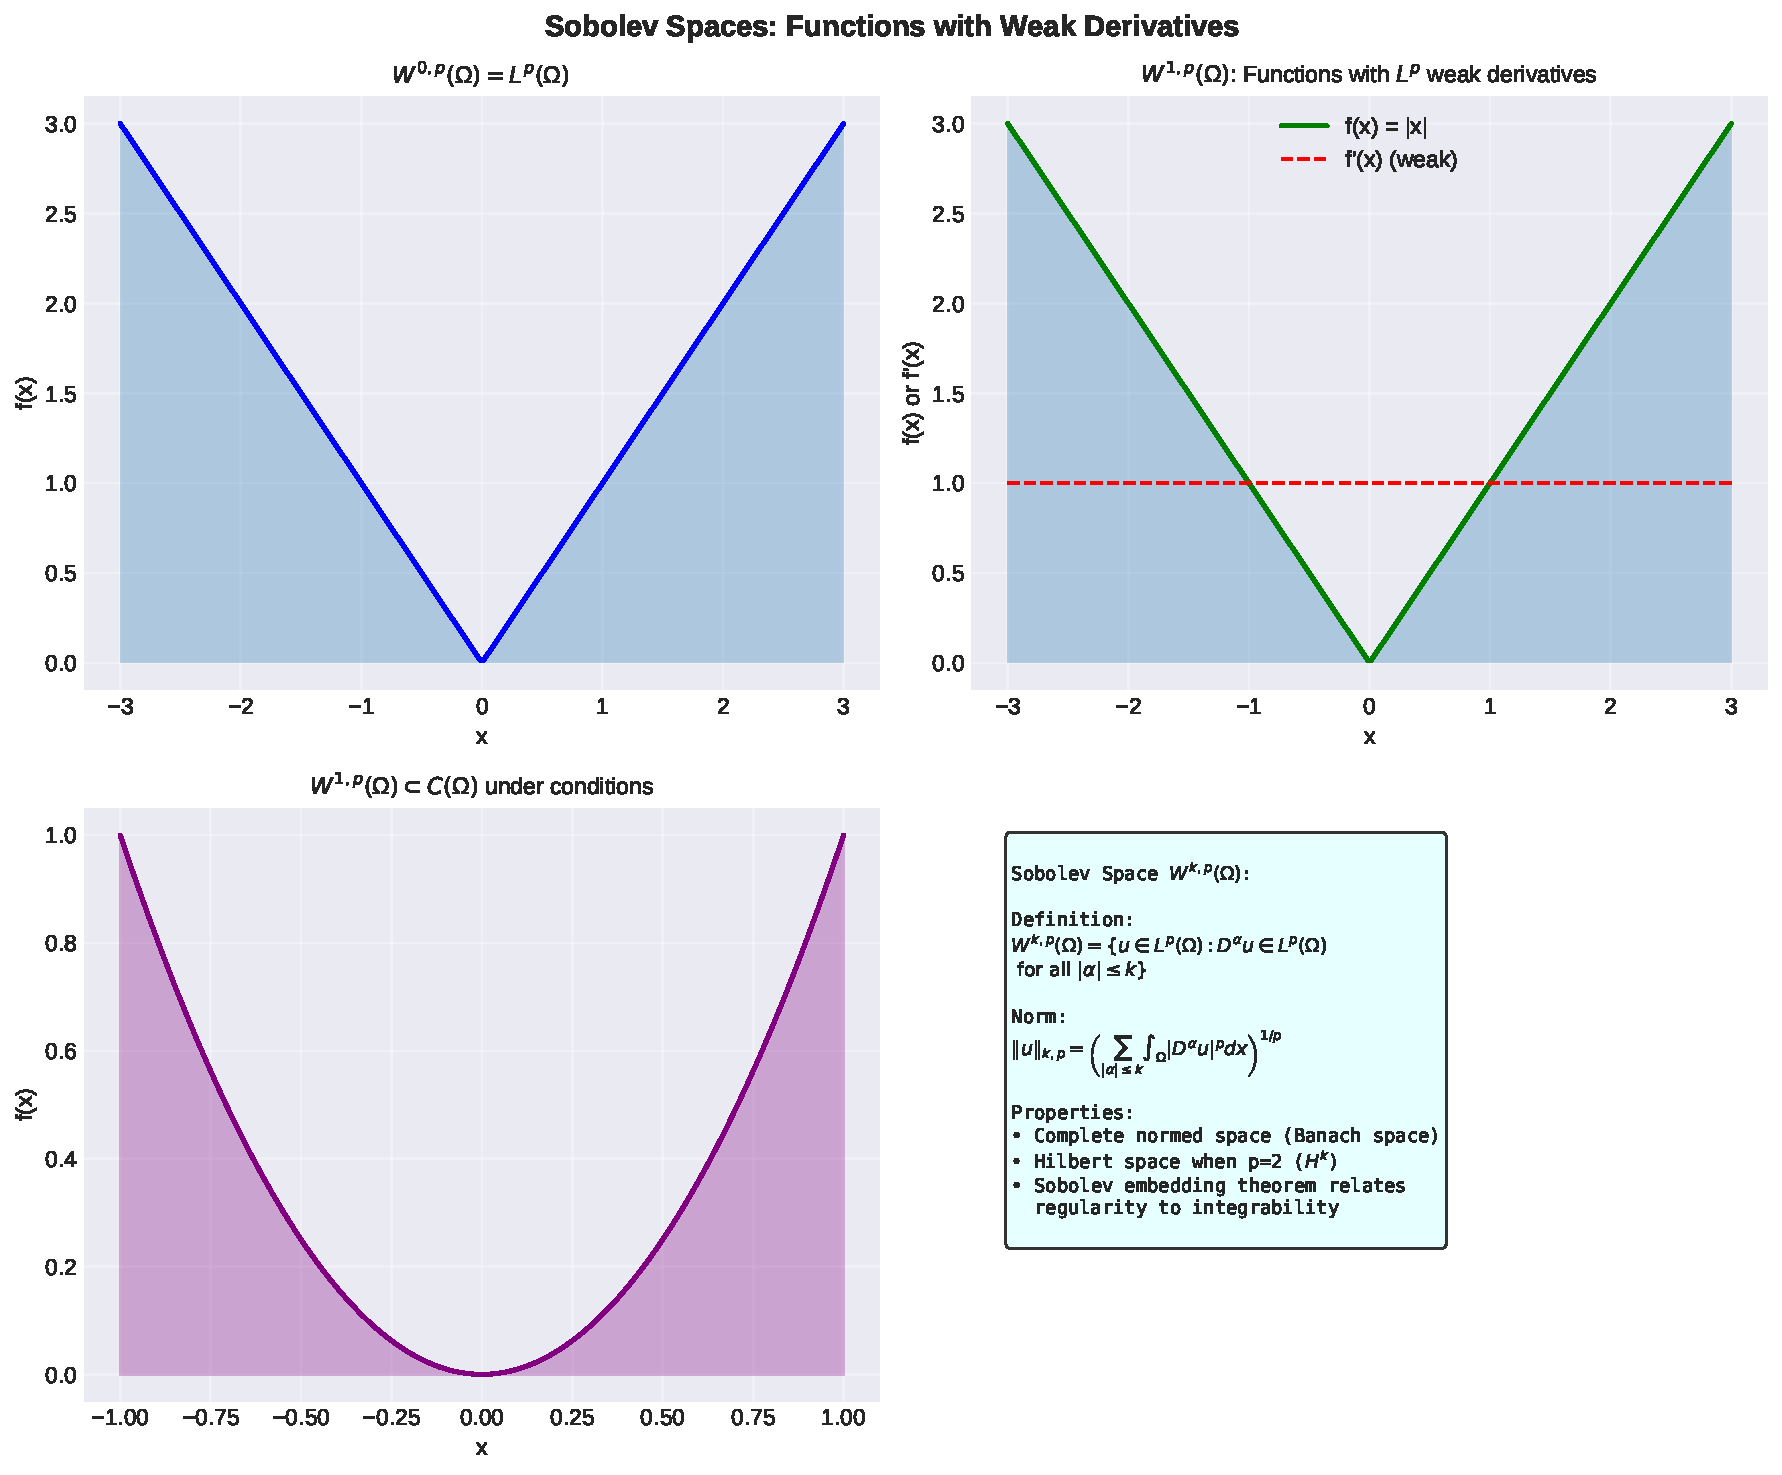
\includegraphics[width=\textwidth]{fig_sobolev_spaces.pdf}
\end{frame}

\begin{frame}{Sobolev Embedding Theorem}
    \begin{theorem}[Sobolev Embedding Theorem]
        Let $\Omega \subset \mathbb{R}^n$ be a bounded open set with smooth boundary. Then:

        \begin{enumerate}
            \item If $0 \leq l < k$ and $\frac{1}{r} \geq \frac{1}{p} - \frac{k-l}{n}$, then
            \[
                W^{k,p}(\Omega) \subset W^{l,r}(\Omega)
            \]
            with continuous embedding. The embedding is compact if $\frac{1}{r} > \frac{1}{p} - \frac{k-l}{n}$.

            \item If $\frac{1}{p} - \frac{k}{n} > 0$, then $W^{k,p}(\Omega) \subset C^\alpha(\Omega)$ for some $\alpha > 0$

            \item If $\frac{1}{p} - \frac{k}{n} = 0$, then $W^{k,p}(\Omega) \subset L^q(\Omega)$ for all $q < \infty$
        \end{enumerate}
    \end{theorem}

    \vspace{0.3cm}
    \small
    \textbf{Key takeaway:} Sobolev spaces allow us to gain continuity by trading regularity for integrability.
\end{frame}

% ============================================================================
% Section 7: Key Theorems
% ============================================================================
\section{Key Theorems and Results}

\begin{frame}{Theorem 1.40: Carathéodory Superposition}
    \begin{theorem}[Theorem 1.40: Continuous Nemytski Operator]
        Let $f: \Omega \times \mathbb{R} \to \mathbb{R}$ be a Carathéodory function satisfying:
        \[
            |f(s, x)| \leq a(s) + b|x|^{p/q}
        \]
        where $a \in L_q(\Omega)$, $b \geq 0$, and $\frac{1}{p} + \frac{1}{q} = 1$.

        Then the superposition operator $F_f(x)(s) = f(s, x(s))$ is continuous and bounded from $L_p(\Omega)$ to $L_q(\Omega)$.
    \end{theorem}

    \vspace{0.3cm}
    \textbf{Application:} If $x_n \to x$ in $L_p$, then $F(x_n) \to F(x)$ in $L_q$
\end{frame}

\begin{frame}{Theorem 1.41: Superposition on $L_1$}
    \begin{theorem}[Theorem 1.41: Superposition on $L_1$]
        Assume $f: \Omega \times \mathbb{R} \to \mathbb{R}$ satisfies the Carathéodory conditions and:
        \[
            |f(s, x)| \leq a(s) + b|x|
        \]
        where $a \in L_1(\Omega)$ and $b \geq 0$.

        Then the superposition operator $F_f$ maps $L_1(\Omega)$ into itself and is continuous.
    \end{theorem}

    \vspace{0.3cm}
    \textbf{Special case:} Linear growth in $x$ ensures mapping from $L_1$ to $L_1$
\end{frame}

\begin{frame}{Theorem 1.44: Continuous Functions on Compact Sets}
    \begin{theorem}[Theorem 1.44: Nemytski Operator on Continuous Functions]
        Let $f: \Omega \times \mathbb{R} \to \mathbb{R}$ be continuous as a map from $\Omega \times \mathbb{R} \to \mathbb{R}$, where $\Omega \subset \mathbb{R}^n$ is a closed and bounded subset.

        Then the superposition operator $F_f$ acts on $C(\Omega)$ (space of continuous functions) and is continuous and bounded.
    \end{theorem}

    \vspace{0.3cm}
    \textbf{Connection:} Extends Carathéodory results to the space $C(\Omega)$
\end{frame}

\begin{frame}{Theorem 1.49: Sobolev Embedding}
    \begin{theorem}[Theorem 1.49: Sobolev Embedding Theorem]
        Let $\Omega \subset \mathbb{R}^n$ be a bounded open set with smooth boundary. Then:

        \begin{enumerate}
            \item If $0 \leq l < k$ and $\frac{1}{r} \geq \frac{1}{p} - \frac{k-l}{n}$, then
            \[
                W^{k,p}(\Omega) \subset W^{l,r}(\Omega)
            \]
            with continuous embedding (compact if strict inequality).

            \item If $\frac{1}{p} - \frac{k}{n} < 0$, then $W^{k,p}(\Omega) \subset C^{0,\alpha}(\Omega)$
        \end{enumerate}
    \end{theorem}
\end{frame}

% ============================================================================
% Section 8: Applications
% ============================================================================
\section{Applications}

\begin{frame}{Application 1: Existence of Solutions to Integral Equations}
    \textbf{Problem:} Consider the Urysohn integral equation
    \[
        u(s) = \int_\Omega K(s, t, u(t)) \, dt + f(s)
    \]

    \vspace{0.3cm}
    \textbf{How Continuous Functions Help:}
    \begin{enumerate}
        \item View the right-hand side as a superposition operator
        \item Use Carathéodory conditions on $K(s, t, u)$
        \item Prove operator is continuous and compact
        \item Apply Schauder fixed-point theorem
    \end{enumerate}

    \vspace{0.3cm}
    \textbf{Conclusion:} Equation has at least one solution
\end{frame}

\begin{frame}{Application 2: Nonlinear Differential Equations}
    \textbf{Problem:} Existence of solutions to
    \[
        \begin{cases}
            u'(t) = f(t, u(t)) \\
            u(0) = u_0
        \end{cases}
    \]

    \vspace{0.3cm}
    \textbf{How Continuous Functions Help:}
    \begin{enumerate}
        \item Rewrite as integral equation: $u(t) = u_0 + \int_0^t f(s, u(s)) \, ds$
        \item Carathéodory conditions ensure the integral is well-defined
        \item Operator is continuous and maps appropriate space to itself
        \item Apply Banach fixed-point theorem or Brouwer's theorem
    \end{enumerate}

    \vspace{0.3cm}
    \textbf{Picard-Lindelöf Theorem:} If $f$ is Lipschitz in $u$, then unique solution exists
\end{frame}

\begin{frame}{Application 3: Sobolev Spaces in PDE}
    \textbf{Problem:} Weak formulation of boundary value problem
    \[
        \begin{cases}
            -\Delta u = f(x) & \text{in } \Omega \\
            u = 0 & \text{on } \partial\Omega
        \end{cases}
    \]

    \vspace{0.3cm}
    \textbf{How Sobolev Spaces Help:}
    \begin{enumerate}
        \item Seek weak solutions in $u \in H_0^1(\Omega) = W_0^{1,2}(\Omega)$
        \item Weak formulation: $\int_\Omega \nabla u \cdot \nabla v \, dx = \int_\Omega f v \, dx$ for all test functions
        \item Use Lax-Milgram theorem (requires Hilbert space structure)
        \item Sobolev embedding gives regularity of solution
    \end{enumerate}

    \vspace{0.3cm}
    \textbf{Result:} Unique weak solution exists and belongs to $H^1(\Omega)$
\end{frame}

\begin{frame}[fragile]{Application Example: Solving an ODE Numerically}
    \begin{lstlisting}[language=Python]
import numpy as np
from scipy.integrate import odeint

# ODE: u'(t) = f(t, u(t))
def f(u, t):
    """Carathéodory function f(t,u) = sin(t) * u^2"""
    return np.sin(t) * u**2

# Initial condition
u0 = 1.0

# Time grid
t = np.linspace(0, np.pi, 100)

# Solve using odeint
# Uses continuous functions internally
u_solution = odeint(f, u0, t)

# Verify: Plot solution
import matplotlib.pyplot as plt
plt.plot(t, u_solution)
plt.xlabel('t')
plt.ylabel('u(t)')
plt.title("Solution to u'(t) = sin(t)*u^2")
plt.grid(True)
plt.show()
    \end{lstlisting}
\end{frame}

% ============================================================================
% Section 9: Summary and Conclusion
% ============================================================================
\section{Summary and Conclusion}

\begin{frame}{Key Takeaways}
    \begin{itemize}
        \item \textbf{Continuous functions} are fundamental objects preserving limits and providing natural structure for analysis

        \item \textbf{Carathéodory functions} extend continuity to product spaces with growth conditions

        \item \textbf{Superposition operators} (Nemytski) are continuous under Carathéodory conditions and growth bounds

        \item \textbf{Uniform continuity} on compact sets ensures boundedness and attainment of extrema

        \item \textbf{Sobolev spaces} extend the notion of continuity via weak derivatives, essential for modern PDE theory

        \item These concepts are \textbf{interdependent}: continuity $\Rightarrow$ compactness $\Rightarrow$ uniform continuity
    \end{itemize}
\end{frame}

\begin{frame}{Further Reading}
    \small
    \textbf{From Pathak's Text:}
    \begin{itemize}
        \item Chapter 1.6--1.9: Measure theory, Sobolev spaces, elliptic operators
        \item Chapter 3: Gâteaux and Fréchet derivatives
        \item Chapter 4: Monotone and maximal operators
        \item Chapter 5--6: Fixed point theorems and topological degree
    \end{itemize}

    \vspace{0.3cm}
    \textbf{Related References:}
    \begin{itemize}
        \item \textit{Functional Analysis} by Rudin (classical treatment)
        \item \textit{Nonlinear Functional Analysis} by Deimling (applications)
        \item \textit{The Sobolev Spaces in Mathematics and Their Applications}
    \end{itemize}

    \vspace{0.3cm}
    \textbf{Key Researchers Mentioned:}
    \begin{itemize}
        \item Carathéodory (continuous functions)
        \item Nemytski (superposition operators)
        \item Sobolev (function spaces)
        \item Krasnoselskii (nonlinear operators)
    \end{itemize}
\end{frame}

\begin{frame}{Final Remarks}
    \begin{center}
        \Large\textbf{Continuous Functions: The Bridge Between Analysis and Applications}
    \end{center}

    \vspace{0.5cm}
    Continuous functions provide the natural setting for:
    \begin{itemize}
        \item Rigorous analysis of functions and operators
        \item Existence and uniqueness of solutions to differential equations
        \item Approximation theory and numerical analysis
        \item Optimization and variational problems
    \end{itemize}

    \vspace{0.5cm}
    The theory of continuous functions is \textbf{complete}, \textbf{elegant}, and \textbf{powerful}---essential for modern mathematics and applications.
\end{frame}

\end{document}
